\documentclass{standalone}
\usepackage{amsmath, amsthm, amssymb, amsbsy}
\usepackage{textgreek, upgreek, gensymb, mathtools, extarrows}
\usepackage{tikz}
\usetikzlibrary{patterns,matrix,positioning,shapes}
\begin{document}
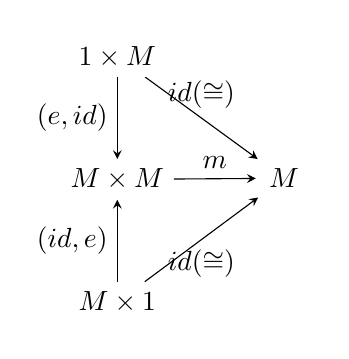
\begin{tikzpicture}
   \matrix (m) [matrix of math nodes,
              row sep=3em, column sep=3em, minimum width=2em]{
    1 \times M & \\
    M \times M & M \\
    M \times 1 & \\};
 \path[-stealth]
   (m-1-1) edge node [above] {$id(\cong)$} (m-2-2)
   (m-1-1) edge node [left] {$(e, id)$} (m-2-1)
   (m-2-1) edge node [above] {$m$} (m-2-2)
   (m-3-1) edge node [left] {$(id, e)$} (m-2-1)
   (m-3-1) edge node [below] {$id(\cong)$} (m-2-2);
\end{tikzpicture}
\end{document}
